\documentclass[12pt]{article}
\usepackage{design_ASC}
\usepackage[T2A]{fontenc}
\usepackage[utf8]{inputenc}
\usepackage[russian]{babel}
\usepackage{hyphenat}
\hyphenation{ма-те-ма-ти-ка вос-ста-нав-ли-вать}

\setlength\parindent{0pt}

\title{Типовой расчет по матиематике\\Кратные, криволинейные и поверхностные интегралы. Теория поля\\4 модуль}

\author{ФИО\\
Студент группы P3113\\
\textsc{Вариант №}}

\begin{document}
\setlength{\droptitle}{-5em}    

\maketitle

\subsection*{I. Плоская область D ограничена заданными линиями.}

$y=\sqrt{x}, x+y=2, x-y=2$\vspace{2.5mm}

1) Сделайте схематический рисунок области D.

\begin{figure}[ht!]
	\centering
	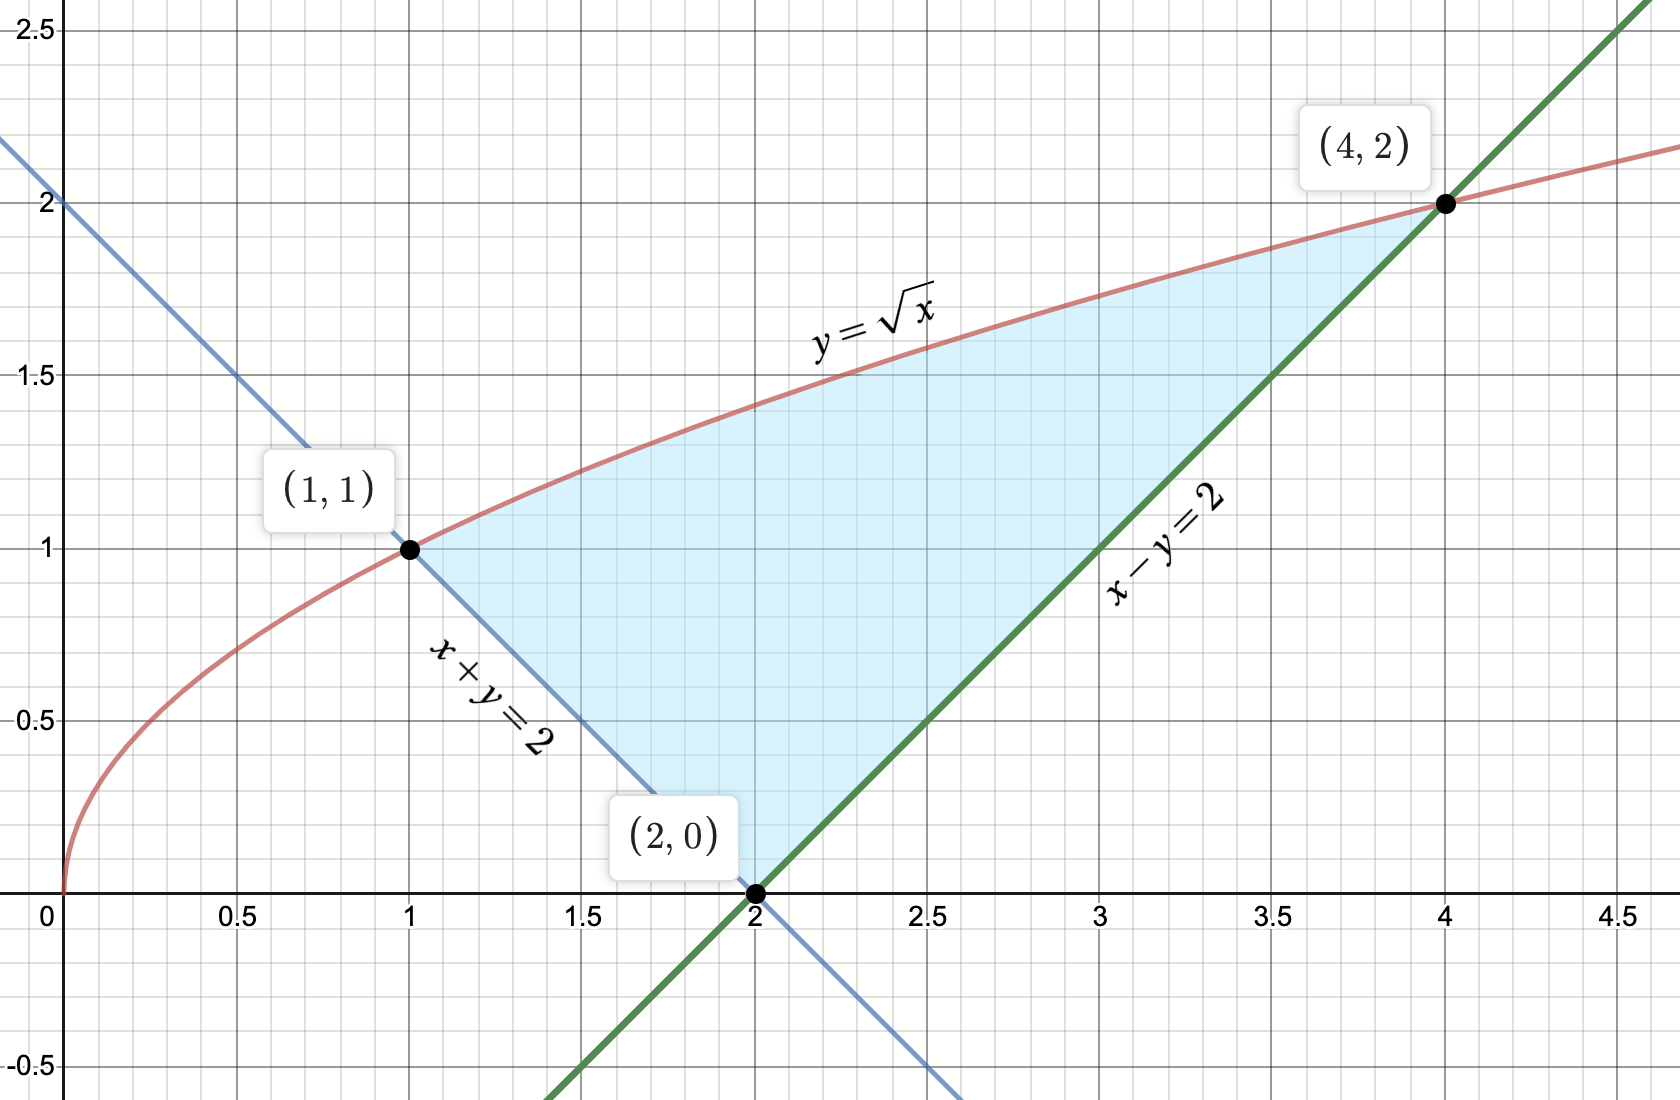
\includegraphics[width=300pt]{Figures/1.png}
\end{figure}

2) С помощью двойного интеграла найдите площадь области D. 

$S=\iint\limits_{D} d x d y=\iint\limits_{D_{1}} d x d y+\iint\limits_{D_{2}} d x d y=\int\limits^{2}_{1}dx\int\limits^{\sqrt {x}}_{2-x}dy+\int\limits^{4}_{2}dx\int\limits^{\sqrt {x}}_{x-2}dy=\int_{1}^{2}(\sqrt{x}-(2-x)) d x+\\+\int_{2}^{4}(\sqrt{x}-(x-2)) d x=\int_{1}^{2} x d x+\int_{1}^{2} \sqrt{x} d x-2 \int_{1}^{2} 1 d x+=-\int_{2}^{4} x d x+\int_{2}^{4} \sqrt{x} d x+2 \int_{2}^{4} 1 d x=\vspace{2.5mm}\\=\frac{1}{6}(8 \sqrt{2}-7)+\frac{2}{3}(5-2 \sqrt{2})=2\frac{1}{6}$\vspace{2.5mm}

Ответ: $2\frac{1}{6}$\vspace{2.5mm}

\subsection*{II. Тело Т ограничено заданными поверхностями.}

$z=\frac{x^{2}+y^{2}}{4}+1, z=\frac{3\left(x^{2}+y^{2}\right)}{4}-1, x=0, y=0 \text { при }x \geq 0, y \geq 0$\vspace{2.5mm}

1) Сделайте схематический рисунок тела Т.

\begin{figure}[ht!]
	\centering
	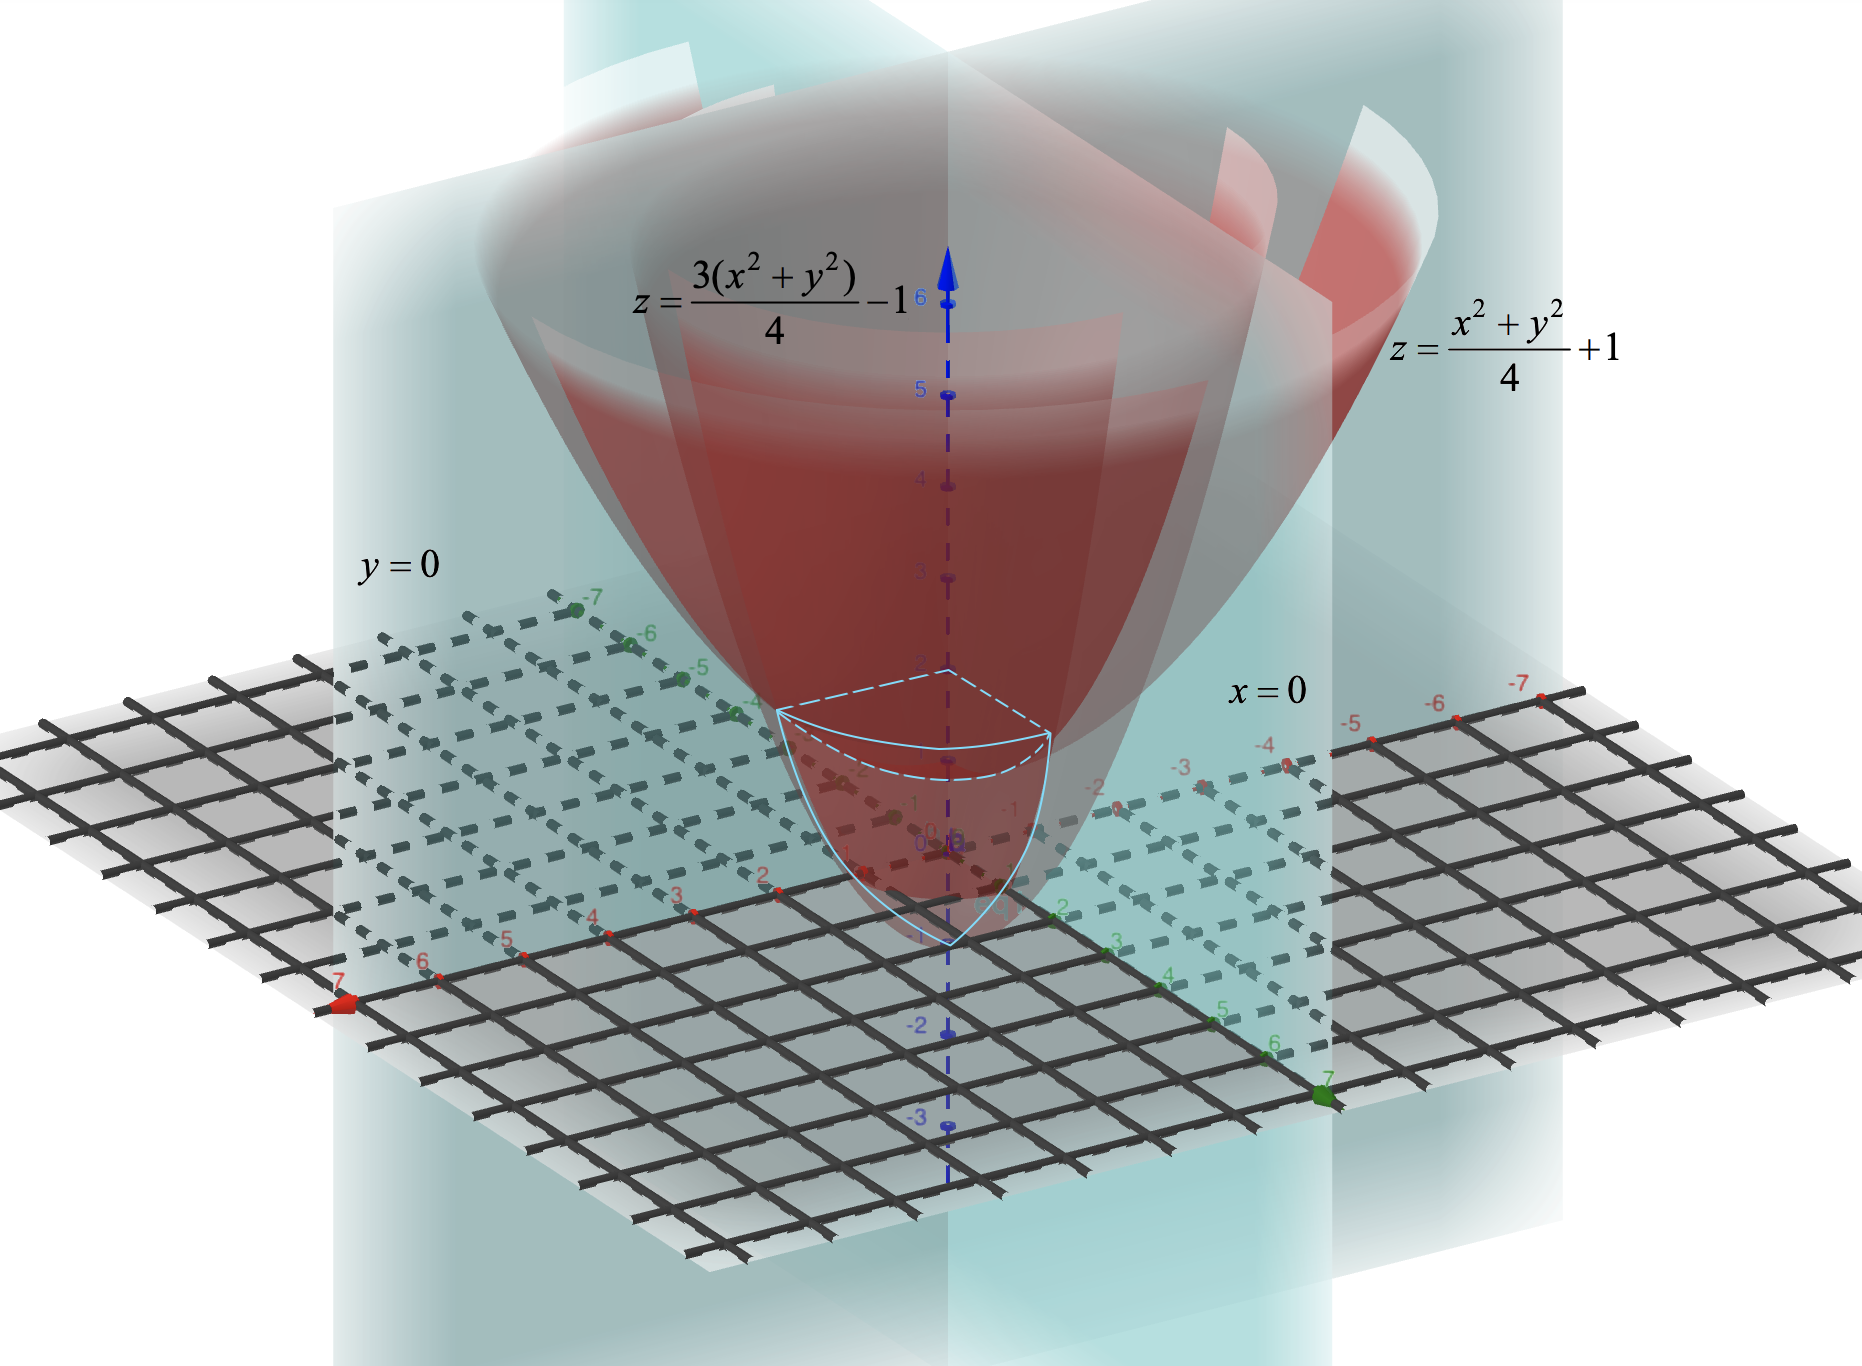
\includegraphics[width=\textwidth]{Figures/2.png}
\end{figure}

2) С помощью тройного интеграла найдите объем тела Т,
перейдя к цилиндрическим или сферическим координатам. 

$=$\vspace{2.5mm}

Ответ: $ $\vspace{2.5mm}

\subsection*{III. С помощью криволинейного интеграла первого рода
найдите массу M дуги плоской материальной кривой, заданной уравнениями а) $y=f(x)$ при $x_{1} \leq x \leq x_{2}$ б) $\left\{\begin{array}{l} x=\varphi(t) \\ y=\psi(t) \end{array}\right.$ $t_{1} \leq t \leq t_{2}$, если плотность вещества равна $\rho(x, y)$.}

a) $y=\sin x, \rho(x, y)=y \cos x, x_{1}=0, x_{2}=\frac{\pi}{2}$\vspace{2.5mm}

Ответ: $ $\vspace{2.5mm}

б) $\left\{\begin{array}{c}x=\ln (t+\sqrt{1+t^{2}}) \\ y=\sqrt{1+t^{2}}\end{array}, \rho(x, y)=\frac{1}{y}, t_{1}=0, t_{2}=1\right.$\vspace{2.5mm}

Ответ: $ $\vspace{2.5mm}

\subsection*{IV. С помощью криволинейного интеграла первого рода
найдите массу M дуги пространственной материальной кривой, заданной уравнениями $\left\{\begin{array}{l}x=\varphi(t) \\ y=\psi(t)$ при $t_{1} \leq t \leq t_{2} \\ z=\chi(t)\end{array}\right.$, если плотность вещества равна $\rho(x, y, z)$.}

$\left\{\begin{array}{l}x=4 \sin t \\ y=3 t \quad, \rho(x, y, z)=\frac{y}{x^{2}+y^{2}+z^{2}}, t_{1}=0, t_{2}=4 \\ z=4 \cos t\end{array}\right.$\vspace{2.5mm}

Ответ: $ $\vspace{2.5mm}

\subsection*{V. Дано векторное поле $\vec{a}$ и плоскость $\sigma,$ пересекающая координатные плоскости по замкнутой ломаной $K L M K,$ где $K$ $L, M-$ точки пересечения плоскости $\sigma$ с координатными осями $O x, O y, O z$ соответственно.}

$\vec{a}=(x+y) \vec{i}+(z-2) \vec{k}, \sigma: 2 x+2 y-3 z=6$\vspace{2.5mm}

1) Найдите поток $Q$ векторного поля $\vec{a}$ через часть $S$ плоскости $\sigma,$ вырезанной координатными плоскостями, в сторону нормали $\vec{n},$ направленной от начала координат $O(0; 0; 0)$\\



2) С помощью теоремы Остроградского-Гаусса найдите поток $Q$ векторного поля $\vec{a}$ через полную поверхность тетраэдра $ОLМК$ в сторону внешней нормали.\\



3) Найдите циркуляцию $C$ векторного поля $\vec{a}$ по контуру $K L M K$, образованному пересечением плоскости $\sigma$ с координатными плоскостями.\\

\subsection*{VI. Дано векторное поле $\vec{a}(M)$.}

$\vec{a}=(2 x y+2) \vec{i}+\left(x^{2}-2 y z-y^{2}\right) \vec{j}+\left(z^{2}-y^{2}\right) \vec{k}$\vspace{2.5mm}

1) Проверьте, является ли векторное поле соленоидальным или потенциальным.\\



2) Если поле потенциально, найдите его потенциал.\\\



\end{document}